\chapter{点云语义分割主动域适应相关理论基础}
\thispagestyle{others}
\pagestyle{others}
\xiaosi
% 文字其实总共,包括引言和小结也就6-7页,先写后补
\section{本章引言}
本章节对本文研究相关的各个领域理论基础进行介绍,包含点云语义分割基础知识、 主动学习基础知识以及域适应相关知识。对于点云语义分割,主要介绍常用点云表示方式,点云语义分割任务的基本任务模型以及评价指标;对于主动学习,介绍主动学习的基本概念及其流程框架;对于域适应部分,主要对域适应概念及域对齐的常见方法进行了介绍。最后,对点云语义分割域适应相关任务中常用公开数据集进行了介绍。

\section{点云语义分割相关知识}
\subsection{三维点云理论基础}
三维点云是三维空间中离散点的集合,每个点通过坐标$(x, y, z)$描述位置,部分还包含颜色、反射强度等附加信息。这些点通常由激光雷达(LiDAR)、深度相机等设备采集而来,能够高精度还原物体表面的几何特征。与传统的二维图像不同,点云直接记录三维空间信息,因此在机器人导航、自动驾驶、虚拟现实等领域有不可替代的作用。如图\ref{fig:2-1}所示,点云数据根据采集场景可分为室内与室外两类。室内点云多由深度相机或近距离激光雷达获取,特点是密度高、遮挡少,适合精细建模。例如扫地机器人通过室内点云构建房间地图,避开桌椅等障碍物。室外点云则依赖车载或机载激光雷达,场景尺度大,但点云稀疏且包含动态物体。自动驾驶汽车利用这类数据识别远处的车辆、行人,但需要处理树木遮挡或雨天噪声的干扰。尽管场景不同,两类点云均需应对数据量大、无序排列和非结构化的共性挑战。  
% 点云的获取方式主要包括主动式和被动式两类。主动式传感器如激光雷达通过发射激光束并计算反射时间生成点云,精度高但成本昂贵,多用于室外测绘或自动驾驶。被动式技术如多视角立体视觉,依靠多个摄像头拍摄二维图像后重建三维点云,成本低但依赖光照条件,适合室内小物体建模。近年来,消费级深度相机(如Kinect)的普及降低了点云采集门槛,推动了室内AR/VR应用的发展。 

点云的优势在于其真实的三维几何表达能力。例如在建筑测绘中,点云能直接输出墙壁的倾斜角度或梁柱的尺寸,而无需从二维图像中推算。同时,点云对光照变化不敏感,在黑暗环境中仍可依靠几何信息工作。然而,点云数据也存在明显缺陷。单帧激光雷达点云可能包含数十万个点,存储与计算成本高昂;传感器噪声或物体遮挡会导致数据缺失,影响后续处理。%此外,点云的无序性使得传统图像处理算法难以直接适用,需依赖PointNet等专门设计的深度学习模型。  
因此,在数据处理层面,点云通常经历去噪、配准、特征提取等步骤。去噪用于消除传感器误差或环境干扰产生的离群点;配准将多视角点云对齐,形成完整场景模型;特征提取则从点云中识别平面、边缘等结构,为物体检测提供基础。随着技术进步,轻量化传感器与实时处理算法逐渐成为趋势。例如自动驾驶系统需在毫秒级时间内完成点云分割,区分道路、车辆与行人。%未来,点云技术可能进一步与AI结合,实现遮挡补全、动态场景预测等功能,但也面临数据压缩、跨场景泛化等挑战。  

点云与其他三维表示方法各有优劣,相比网格(Mesh)模型,点云保留原始采集数据,但缺乏明确的表面连接关系;与体素(Voxel)相比,点云内存占用低且分辨率高,但难以直接应用卷积操作。因此,一般在大规模场景中,往往更多的是选择体素方式进行点云处理。%这种差异使得点云更适用于高精度测量与实时感知,而网格和体素则在渲染、仿真等场景更具优势。理解这些特点有助于在不同任务中选择合适的三维表达方式。  
% 总体而言,点云技术正推动着数字化世界的构建。从自动驾驶汽车识别路况,到元宇宙中虚拟场景的生成,点云在精确空间建模中的作用愈发重要。然而,如何高效处理海量点云数据,仍是学术界与工业界共同探索的方向。
\vspace{-0.1cm}
\begin{figure}[h]
    \centering
    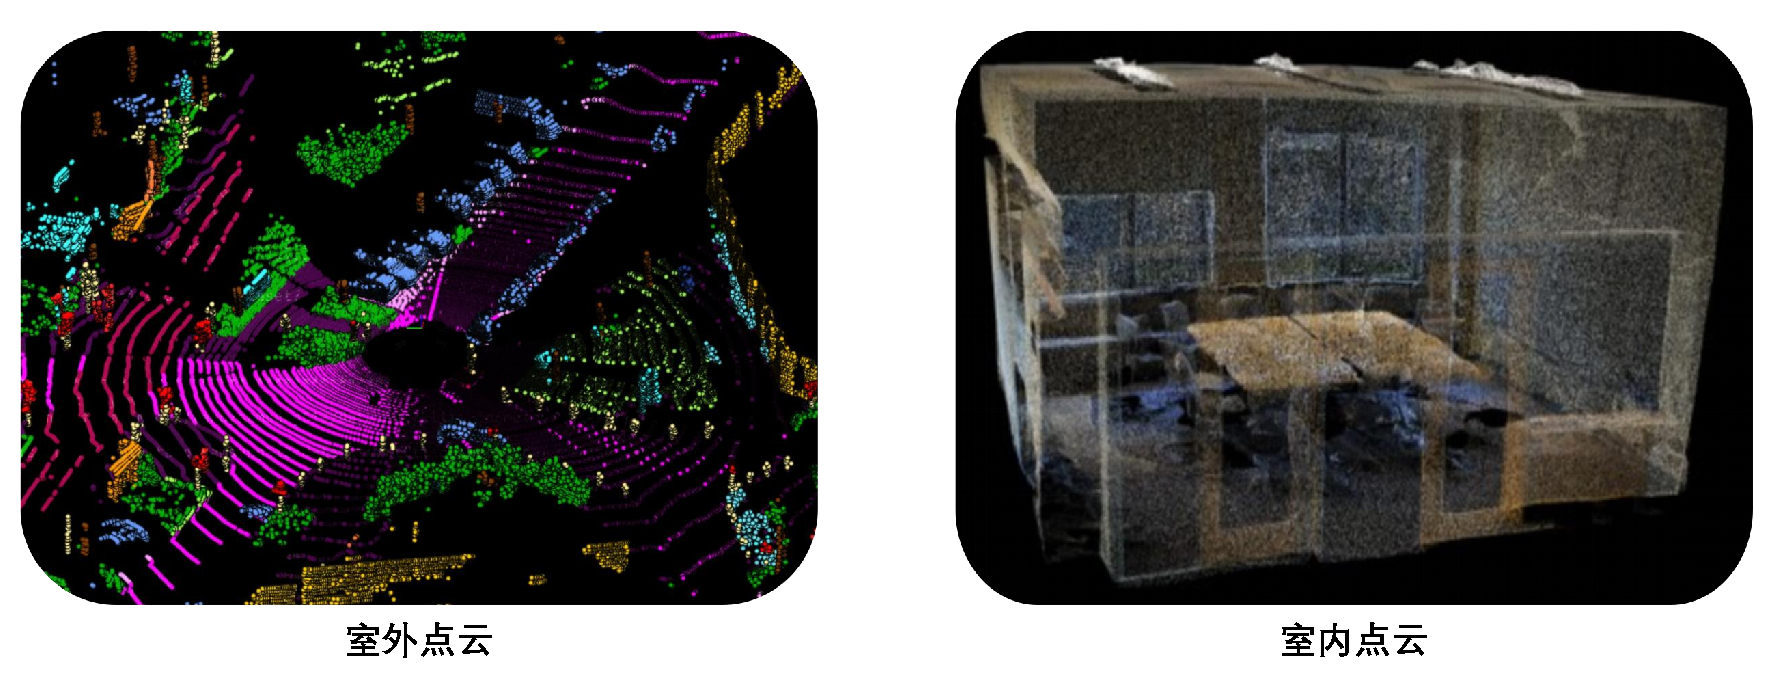
\includegraphics[width = \textwidth, scale=0.5]{ljx/figure/2-1PC.pdf}
    \bicaption[\xiaosi 3D点云]{\wuhao 3D点云}{\wuhao 3D point cloud}
    \label{fig:2-1}
\end{figure}
\vspace{-0.35cm}
\subsection{点云语义分割方法}
\subsubsection{目标与输入数据}
点云语义分割的目标是为三维空间中的每个点赋予特定语义标签。在自动驾驶场景中区分道路、车辆、行人等类别,在室内建模中识别墙面、家具等物体。这一过程本质上是将无序的三维点云转化为带有语义信息的数据。输入的数据通常是由激光雷达或深度相机采集的原始点云,其基础形式为包含$N$个点的坐标矩阵,形状为$N \times 3$,对应每个点的三维坐标$(x, y, z)$。在一些特殊的场景中,点云可能还包含颜色(RGB值)、反射强度(LiDAR返回信号强度)或时间戳(动态场景中的时序信息)等附加特征,此时数据维度扩展为$N \times D$,其中$D \geq 3$。数据预处理阶段通常会对坐标进行归一化,以消除传感器位姿的影响,并对离群点进行滤波以提高后续处理稳定性。

\subsubsection{特征提取方法}
特征提取是点云语义分割的核心,其目的是从原始点云中挖掘具有判别性的局部与全局特征。根据输入表示方式的不同,主流方法可分为三类:

% \subsubsection{基于点的方法}
1)基于点的方法。
此类方法直接处理原始点云,避免因体素化或投影导致的信息损失。典型代表如PointNet++\upcite{qi2017pointnet++},其核心思想是通过多层感知机(MLP)逐点提取特征,并通过最大池化聚合全局信息。具体而言,对于每个点$\mathbf{p}_i$,模型不仅编码其自身坐标,还通过邻域查询(如k近邻或球查询)收集周围点集$\{\mathbf{p}_j \mid j \in \mathbf{N}(i)\}$,进而利用共享权重的$MLP$提取局部几何模式,如公式\eqref{eq:2-1}所示:
\begin{equation}
    \label{eq:2-1}
    \mathbf{F}_i = MLP\left(\mathbf{p}_i - \mathbf{p}_j, \|\mathbf{p}_i - \mathbf{p}_j\|_2\right) \quad \forall j \in \mathbf{N}(i)
\end{equation}
式中,$\mathbf{p}_i - \mathbf{p}_j$表示相对位置;$\|\cdot\|_2$为欧氏距离。通过堆叠多个局部特征提取层,模型可逐步扩大感受野,捕获多尺度几何结构。

% \subsubsection{基于体素的方法}
2)基于体素的方法。
基于体素的方法通过将点云转换为规则三维网格实现高效计算。MinkowskiNet\upcite{MinkowskiNet}是该领域的一个代表性方法,其核心是通过稀疏卷积网络,仅对非空体素进行计算,大幅减少内存与计算开销。稀疏卷积的表达式如公式\eqref{eq:2-2}所示:
\begin{equation}
    \label{eq:2-2}
    \mathbf{F}_{\text{out}}(x,y,z) = \sum_{(dx,dy,dz) \in \mathbf{K}} \mathbf{W}(dx,dy,dz) \cdot \mathbf{F}_{\text{in}}(x+dx, y+dy, z+dz)
\end{equation}
式中,$\mathbf{K}$为卷积核覆盖的偏移范围;$\mathbf{W}$为卷积核权重。与传统三维卷积不同,稀疏卷积通过哈希表管理非空体素坐标,仅对有效位置执行计算。%例如,MinkowskiNet将输入表示为稀疏张量(包含坐标$C$与特征$F$两部分),计算时仅遍历存在点的体素位置。体素化的分辨率由超参数控制,通常设为$0.05$米至$0.1$米以平衡精度与效率。

% 稀疏卷积的核心优势体现在两方面:
% \begin{itemize}
%     \item \textbf{计算效率}:跳过空体素的计算,尤其适合室外大场景中稀疏点云(如自动驾驶场景中90\%以上体素为空),计算量可降低至密集卷积的1/10。
%     \item \textbf{内存优化}:通过坐标压缩存储(仅记录非空体素位置),避免存储全分辨率三维网格,内存占用与点云密度而非场景体积线性相关。
% \end{itemize}
% 体素化将点云转换为规则的三维网格,便于应用三维卷积操作。例如,VoxelNet将点云划分为$L \times W \times H$的体素单元,每个单元内点云通过小型MLP编码为特征向量,再通过三维卷积进行特征融合:
% \begin{equation}
%     \mathbf{V}_{l+1}(x,y,z) = \sum_{i,j,k} \mathbf{W}(i,j,k) \cdot \mathbf{V}_l(x+i, y+j, z+k) + \mathbf{b},
% \end{equation}
% 其中$\mathbf{b}$为偏置项。体素化的优势在于计算效率高,尤其适合GPU并行计算,但分辨率的限制可能导致细小物体(如电线杆)的细节丢失。为此,稀疏卷积技术被提出以跳过空体素,减少计算冗余。

% \subsubsection{基于投影的方法}
3)基于投影的方法。
此类方法将三维点云投影至二维平面,复用成熟的图像处理网络。其中RangeNet++\upcite{RangeNet++}将LiDAR点云转换为球面距离图像(Range Image),每个像素对应点的深度与方位角。投影后的二维图像通过改进的二维卷积网络提取特征,如公式\eqref{eq:2-3}所示:
\begin{equation}
    \label{eq:2-3}
    % \mathbf{F}_{l+1}(u,v) = \text{ReLU}\left(\sum_{m,n} \mathbf{K}(m,n) \cdot \mathbf{F}_l(u+m, v+n)\right)
    \mathbf{F}_{l+1}(u,v) = ReLU\left(\sum_{m,n} \mathbf{K}(m,n) \cdot \mathbf{F}_l(u+m, v+n)\right)
\end{equation}
其中$ReLU$为激活函数。投影方法的计算效率较高,但可能因遮挡或投影畸变导致部分三维信息丢失。%为此,部分研究引入多视图融合策略,结合鸟瞰图与前视图提升鲁棒性。

\subsubsection{分类与损失函数}
在特征提取后,模型通过全连接层将$N \times F$维特征映射至$N \times C$维类别得分矩阵,其中$C$为类别总数。Softmax函数将得分转换为概率分布,为每个点分配类别标签,如公式\eqref{eq:2-4}所示:
\begin{equation}
    \label{eq:2-4}
    P(y_i=c) = \frac{e^{\mathbf{z}_{i,c}}}{\sum_{c'=1}^C e^{\mathbf{z}_{i,c'}}}
\end{equation}
其中$\mathbf{z}_{i,c}$表示第$i$个点在第$c$类上的得分。损失函数采用交叉熵损失,衡量预测概率与真实标签的差异,其数学表达式如公式\eqref{eq:2-5}所示:
\begin{equation}
    \label{eq:2-5}
    L = -\frac{1}{N} \sum_{i=1}^N \sum_{c=1}^C y_{i,c} \log P(y_i=c)
\end{equation}
式中,$y_{i,c}$为one-hot编码的真实标签。%针对类别不平衡问题,可采用加权交叉熵损失,为少数类别分配更高权重:
% \begin{equation}
%     \mathbf{L}_{\text{weighted}} = -\frac{1}{N} \sum_{i=1}^N \sum_{c=1}^C w_c \cdot y_{i,c} \log P(y_i=c),
% \end{equation}
% 其中$w_c$与类别频率成反比。此外,动态采样策略(如在训练时对稀少类别点过采样)也被用于缓解数据偏斜。

% \subsubsection{优化挑战与解决方案}
% 点云语义分割面临稀疏性、遮挡与噪声等挑战。例如,在自动驾驶中,远处物体可能仅包含少量点,导致漏检。为此,RandLA-Net提出随机降采样与局部特征聚合策略,在减少计算量的同时保留关键点信息。另一方向是设计轻量化网络(如Cylinder3D),通过柱状分区减少三维卷积计算量,实现实时推理。未来研究可能结合自监督学习,利用未标注数据提升模型泛化能力,或探索多模态融合(如点云与图像融合)以增强语义理解。
% \section{点云语义分割方法}

% \subsubsection{目标与输入数据}
% 点云语义分割的目标是为三维空间中的每个点分配特定语义标签,例如将点标记为树木、建筑物或车辆等类别。输入数据通常是一个包含$N$个点的坐标矩阵,形状为$N \times 3$,分别对应每个点的$x, y, z$坐标。若点云包含颜色或反射强度等附加信息,数据维度扩展为$N \times D$,其中$D$表示特征总数。

% \subsubsection{特征提取方法}
% 特征提取的实现方式根据输入表示分为三类:

% % \subsubsubsection{基于点的方法}
% 1)基于点的方法 
% 直接处理原始点云,利用多层感知机(MLP)对每个点及其邻域进行编码。公式为:
% \begin{equation}
%     \mathbf{F}_i = \text{MLP}\left(\mathbf{p}_i, \{\mathbf{p}_j \mid j \in \mathbf{N}(i)\}\right),
% \end{equation}
% 其中$\mathbf{p}_i$为第$i$个点的坐标,$\mathbf{N}(i)$为其邻域点集合。

% % \subsubsubsection{基于体素的方法}
% 2)基于体素的方法
% 将点云划分为规则三维网格(体素),采用三维卷积提取特征。设体素分辨率为$L \times W \times H$,卷积核尺寸为$k^3$,则特征更新公式为:
% \begin{equation}
%     \mathbf{V}_{l+1}(x,y,z) = \sum_{i,j,k} \mathbf{W}(i,j,k) \cdot \mathbf{V}_l(x+i, y+j, z+k),
% \end{equation}
% 其中$\mathbf{W}$为卷积核权重,$\mathbf{V}_l$为第$l$层体素特征。

% % \subsubsubsection{基于投影的方法}
% 3)基于投影的方法
% 将点云映射到二维平面(如球面投影),使用二维卷积处理。投影后的特征提取公式为:
% \begin{equation}
%     \mathbf{F}_{l+1}(u,v) = \sum_{m,n} \mathbf{K}(m,n) \cdot \mathbf{F}_l(u+m, v+n),
% \end{equation}
% 其中$\mathbf{K}$为二维卷积核,$(u,v)$为投影图像的像素坐标。

% \subsubsection{分类与损失函数}
% 分类阶段将$N \times F$维特征映射到$N \times C$维类别得分,其中$C$为类别数。通过Softmax计算概率分布:
% \begin{equation}
%     P(y_i=c) = \frac{e^{\mathbf{z}_{i,c}}}{\sum_{c'=1}^C e^{\mathbf{z}_{i,c'}}},
% \end{equation}
% 其中$\mathbf{z}_{i,c}$为第$i$个点在第$c$类上的得分。损失函数采用交叉熵:
% \begin{equation}
%     \mathbf{L} = -\frac{1}{N} \sum_{i=1}^N \sum_{c=1}^C y_{i,c} \log P(y_i=c),
% \end{equation}
% 其中$y_{i,c}$为真实标签的one-hot编码。实际应用中需针对类别不平衡问题(如道路点远多于交通灯)优化损失权重或采样策略。当前方法如PointNet++通过局部几何编码提升精度,但对动态遮挡的鲁棒性仍需改进。
\subsection{评价指标}
在点云语义分割任务中,常用的评估指标有两个,一个是总体精度(Overall Accuracy, OA),另一个则是平均交并比(mean Intersection over Union, mIoU)。

总体精度通过计算正确预测点数占总点数的比例,直观反映模型的整体分类能力,其表示式如公式\eqref{eq:2-6}所示:
\begin{equation}
    \label{eq:2-6}
    OA = \frac{TP + TN}{TP + TN + FP + FN}
\end{equation}
式中,$TP$表示正确预测的正例;$TN$为正确预测的反例;$FP$为误判的正例;$FN$为误判的正例。尽管$OA$计算简单,但在点云语义分割中,由于场景中不同类别点数差异显著,如城市道路点占比可能超过50\%,而交通灯可能不足1\%,$OA$易被多数类别主导,这一缺陷使得$OA$难以真实评估模型性能。

平均交并比则通过衡量每个类别的预测区域与真实区域的重叠程度,提供更均衡的评估。对于类别$c$,其交并比计算公式如\eqref{eq:2-7}所示:
\begin{equation}
    \label{eq:2-7}
    IoU_c = \frac{TP_c}{TP_c + FP_c + FN_c}
\end{equation}
式中,$TP_c$为类别$c$的正确预测点数;$FP_c$为误判为$c$的点数;$FN_c$为漏判的$c$类点数。$mIoU$取所有类别$IoU$的平均值,其表达式如公式\eqref{eq:2-8}所示:
\begin{equation}
    \label{eq:2-8}
    mIoU = \frac{1}{C} \sum_{c=1}^C IoU_c
\end{equation}
式中$C$为类别总数。mIoU的核心优势在于其对每个类别的平等关注,即使某一类别的点数极少,其$IoU$值仍能直接影响整体得分,从而迫使模型兼顾所有类别。
% \subsection{指标选择依据}

当前研究普遍以$mIoU$为核心评价指标,主要因其能够克服类别不平衡带来的评估偏差。点云数据中,高频率类别与低频率类别的点数差异可能达到数百倍,若依赖$OA$这类整体指标,模型可能仅通过优化高频类别即可获得高评分,而忽视低频类别的学习,然而对于语义分割任务来说,实现对每一个类别点的精准分割是其目的所在,所以无论低频率类别还是高频率类别都是同等重要。$mIoU$通过独立计算每个类别的重叠率,确保模型在各类别上的表现均被量化,从而更真实地反映其实际分割能力。此外,$mIoU$对边界误差的敏感性也优于$OA$,物体边缘点的误分类会同时增加$FP$和$FN$,导致$IoU$显著下降,而$OA$可能因整体正确率高而掩盖此类局部缺陷。%学术界的共识进一步强化了mIoU的地位,主流数据集(如SemanticKITTI、nuScenes)与竞赛均将其作为基准指标,使得不同模型间的横向对比更具一致性。尽管OA仍可作为辅助指标反映整体正确率,但其局限性导致其在最新研究中逐渐边缘化。例如,某模型OA达到95\%但mIoU仅为50\%,仍会被认为未达到实际应用要求。未来,随着细分场景需求的增加,边界IoU或动态加权mIoU等指标可能被引入,以更精准地评估复杂环境下的分割质量。
\section{主动学习基础知识}
% \section{主动学习方法}
% \subsection{主动学习的概念与目的}
主动学习作为传统机器学习中的一个分支,其核心思想是让模型在训练过程中主动选择对提升性能最有价值的数据进行标注,而非被动接受随机标注的数据。该方法的核心目的是在有限标注成本的约束下,通过主动的数据选择策略,最大化模型的性能。%例如,在医学图像分析中,专家标注每张CT图像可能耗时数小时,主动学习可优先选择那些最可能改善肿瘤检测模型性能的疑难样本进行标注,从而减少总标注量。
% \subsection{主动学习的基本流程}
如图\ref{fig:2-2}所示,主动学习的流程可概括为迭代式的“选择-标注-训练”循环。首先,利用初始标注数据训练一个基础的目标模型。随后,模型对未标注数据进行推理预测,生成预测结果。基于这些预测,通过预设的选择策略,从未标注数据中筛选出对当前模型提升最有价值的候选数据。%例如,不确定性采样会选择模型预测概率接近0.5的样本,因其分类边界模糊,标注后能有效修正模型决策边界。
筛选出的候选数据由标注者即该领域相关专家进行标注,新标注数据与原有标注数据合并后,用于更新模型参数。这一过程持续迭代,直至标注预算耗尽或模型性能趋于稳定。

流程中的核心模块包括选择策略设计以及模型更新机制,%标注数据管理需平衡新旧数据的分布,避免因过度关注特定样本导致模型偏见。
选择策略的优劣直接决定主动学习效率,常见策略包括不确定性采样、多样性采样和委员会查询。不确定性采样:选择模型预测置信度最低的样本;多样性采样:选择代表数据分布多样性的样本,覆盖不同特征空间区域;委员会查询:训练多个模型,选择各模型预测差异最大的样本。模型更新机制一般考虑如何利用这些已标注的高价值目标点来对模型进行微调以充分发挥数据与模型的潜力。%需考虑增量学习与灾难性遗忘的平衡。例如,在深度学习中,可采用弹性权重固化(EWC)等方法,在更新时保护重要参数不被覆盖。
\vspace{-0.1cm}
\begin{figure}[h]
    \centering
    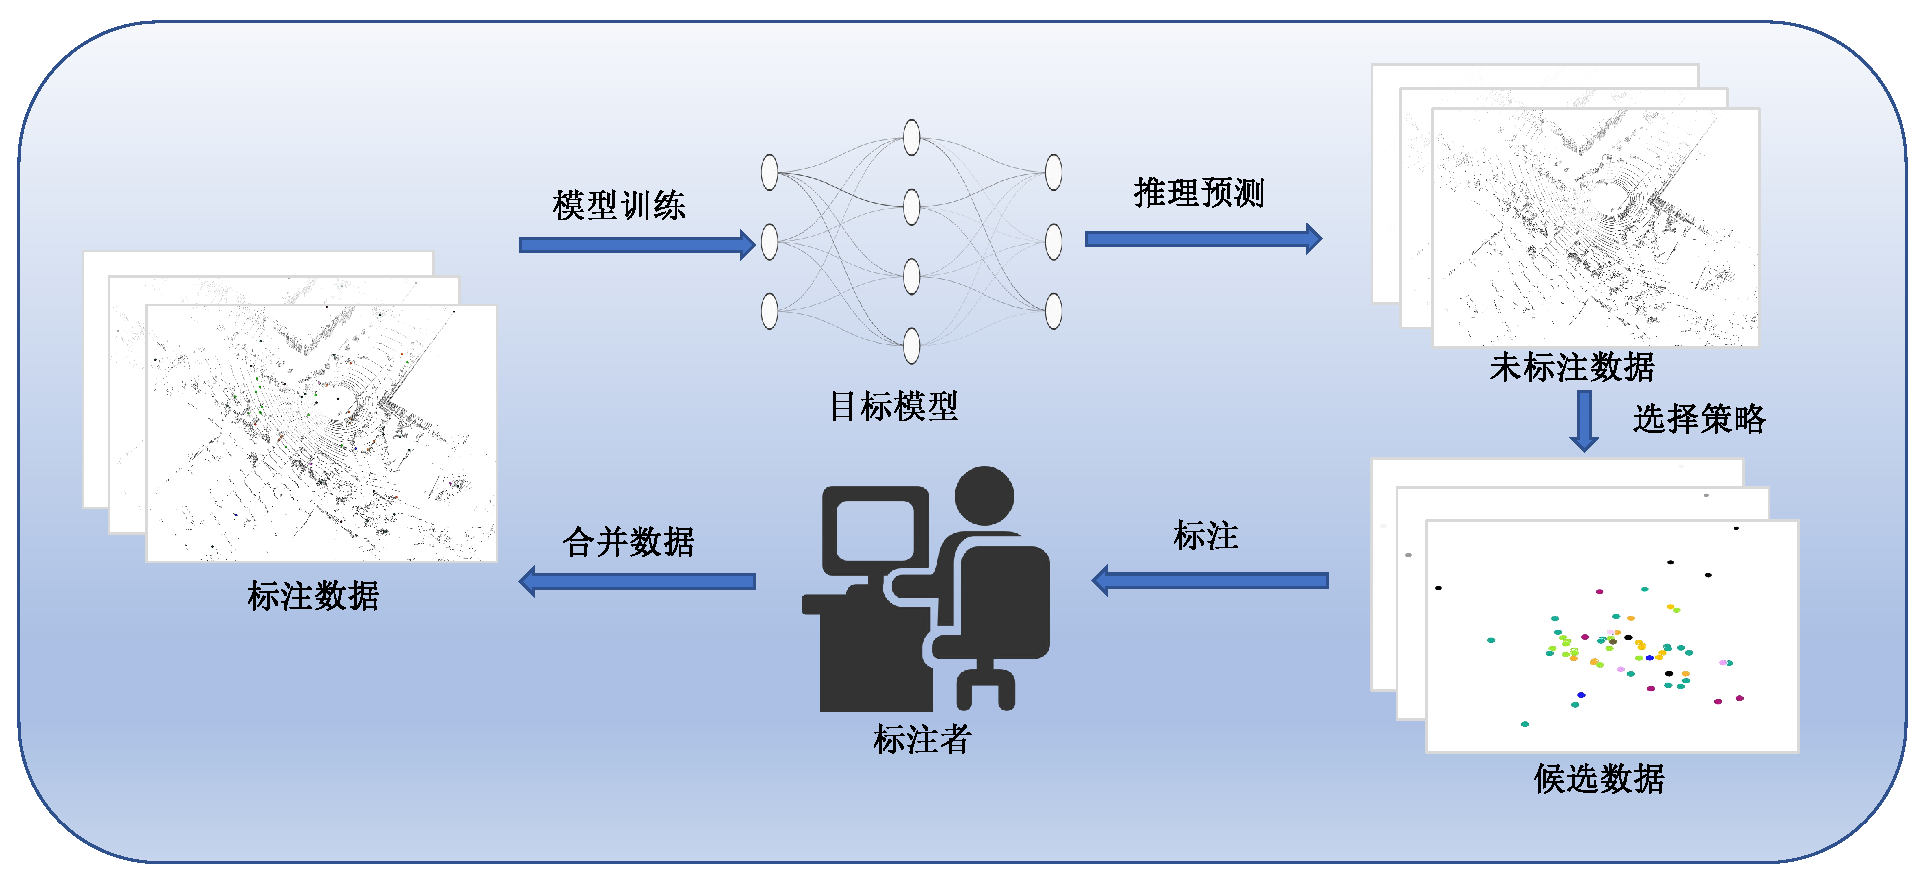
\includegraphics[width = \textwidth, scale=0.5]{ljx/figure/2-2AL.pdf}
    \bicaption[\xiaosi 主动学习]{\wuhao 主动学习}{\wuhao Active learning}
    \label{fig:2-2}
\end{figure}
\vspace{-0.35cm}
% \subsection{应用场景与挑战}
% 主动学习在标注成本高昂或数据分布动态变化的场景中优势显著。例如,自动驾驶中道路标志的标注需适应不同地域、天气条件,主动学习可优先标注罕见场景(如暴雨中的模糊标志)。然而,其挑战在于选择策略的普适性——针对特定任务设计高效策略需领域知识支持。此外,初始模型的质量直接影响后续选择效果,若初始标注数据不足或偏差较大,可能导致选择策略失效。未来研究可能结合自监督预训练,提升初始模型鲁棒性,或设计自适应策略以动态调整选择准则。

\section{域适应基础知识}
% \subsection{域适应的基本概念}
% 域适应(Domain Adaptation)是迁移学习的重要分支,旨在解决源域(Source Domain)与目标域(Target Domain)数据分布不一致导致的模型性能下降问题。假设源域$D_s = \{(x_i^s, y_i^s)\}_{i=1}^{N_s}$包含大量标注数据,而目标域$D_t = \{x_j^t\}_{j=1}^{N_t}$(无监督场景)或少量标注数据$D_t = \{(x_j^t, y_j^t)\}_{j=1}^{N_t}$(半监督场景),域适应的目标是通过对齐两域特征分布,使源域训练的模型$M$能有效泛化至目标域。例如,在自动驾驶中,源域可能为合成点云数据(如CARLA仿真),目标域为真实激光雷达数据,域适应可缩小两者因传感器差异和场景复杂度引起的分布偏移。
% \vspace{-0.1cm}
% \begin{figure}[h]
%     \centering
%     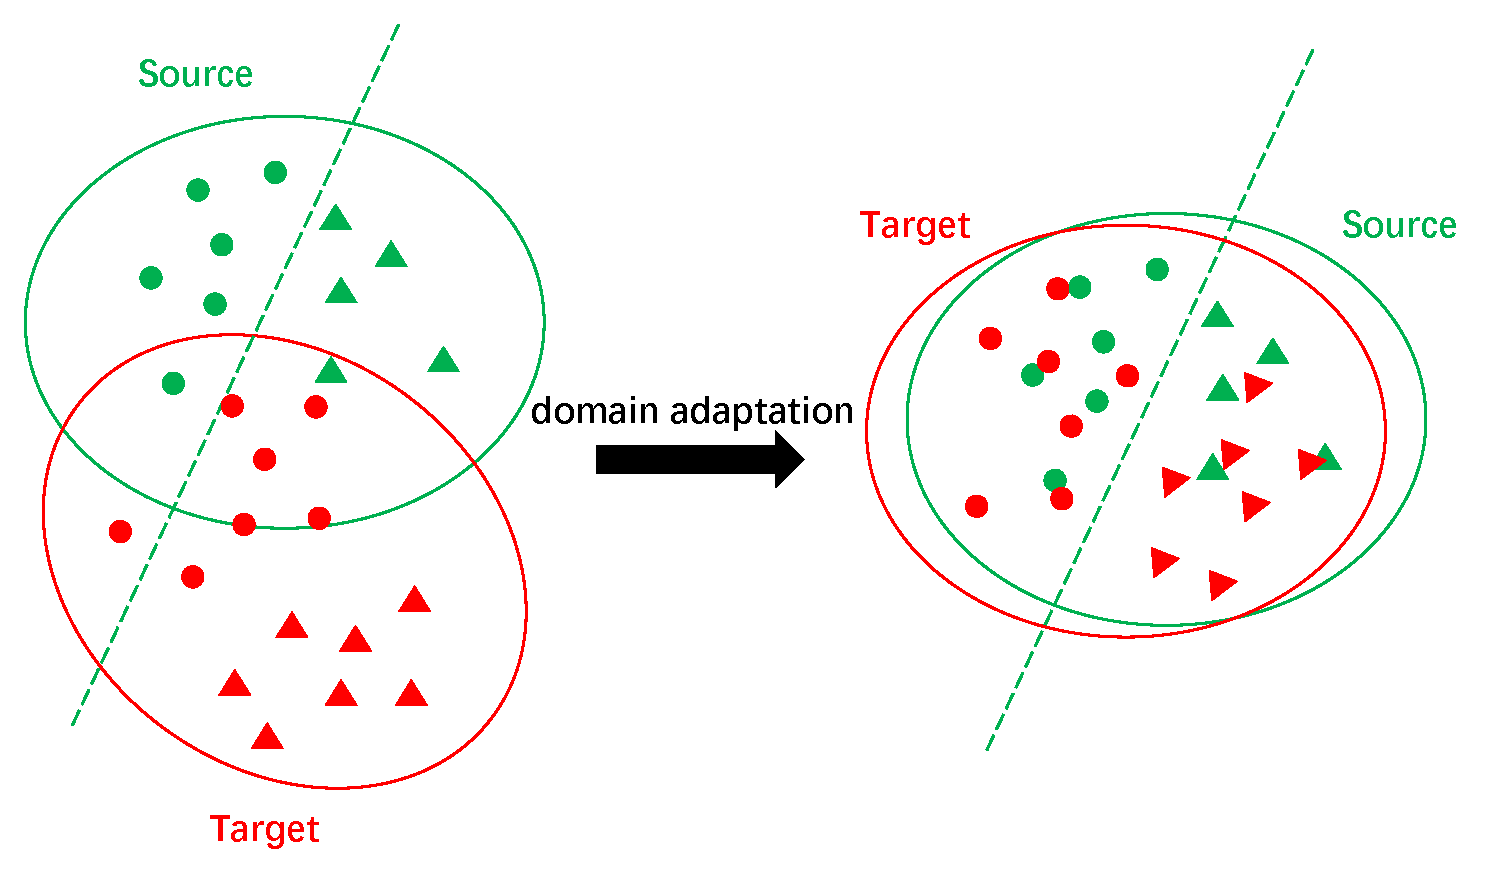
\includegraphics[width = \textwidth, scale=0.5]{ljx/figure/2-3DA.pdf}
%     \bicaption[\xiaosi 域适应]{\wuhao 域适应}{\wuhao Domain adaptation}
%     \label{fig:2-3}
% \end{figure}
% \vspace{-0.35cm}
% \subsection{域适应的核心目标}
% 域适应的核心数学目标是最小化源域与目标域在特征空间中的分布差异,同时保持任务性能(如分类准确率)。定义源域分布为$P_s(x,y)$,目标域分布为$P_t(x,y)$,域适应需实现:
% \begin{equation}
%     \min_{\theta} \underbrace{\mathbb{E}_{(x,y) \sim P_s} \mathbf{L}(f_\theta(x), y)}_{\text{源域任务损失}} + \lambda \cdot \underbrace{d(P_s(x), P_t(x))}_{\text{域差异度量}},
% \end{equation}
% 其中$d(\cdot,\cdot)$为分布距离度量函数,$\lambda$为权衡系数。当目标域无标签时,任务损失仅作用于源域,域对齐成为关键优化方向。
域适应是机器学习中一种重要的技术,主要用于解决模型在相同任务不同数据分布场景下的泛化问题。如图\ref{fig:2-3}所示,当模型在一个数据集即源域上训练得很好,能够正确的将数据分类,但在另一个数据集称为目标域上表现却不佳,无法对目标域中的数据进行正确的分类,而造成这一现象的主要原因是因为不同数据域之间分布不同,存在域间差异,从而导致模型无法对新数据域中的数据进行正确分类,而域适应的目标就是帮助模型适应目标域的数据分布,从而提升其在新数据中的性能。
% 简单来说,当模型在一个数据集即源域上训练得很好,但在另一个数据集称为目标域上表现不佳时,
% 例如,假设我们用一个在晴天采集的自动驾驶点云数据(源域)训练了一个模型,但实际应用中需要处理雨雾天气的点云(目标域),域适应技术可以帮助模型更好地理解雨雾中的障碍物,即使它从未在雨雾数据中直接训练过。
域适应的核心思想是找到源域和目标域之间的共同特征,并通过调整模型或数据,缩小两者之间的分布差异。造成这些差异的原因有很多,比如点云的密度、物体形状的细微变化,或者传感器采集数据的方式不同。
% 举个例子,源域可能是由高精度激光雷达生成的密集点云,而目标域可能来自低成本雷达,点云更稀疏且噪声更多。
域适应的目标就是让模型学会忽略这些差异,而专注于识别共同的特征信息,学习到域不变特征即两域特征子空间知识。
% \vspace{-0.1cm}
\begin{figure}[h]
    \centering
    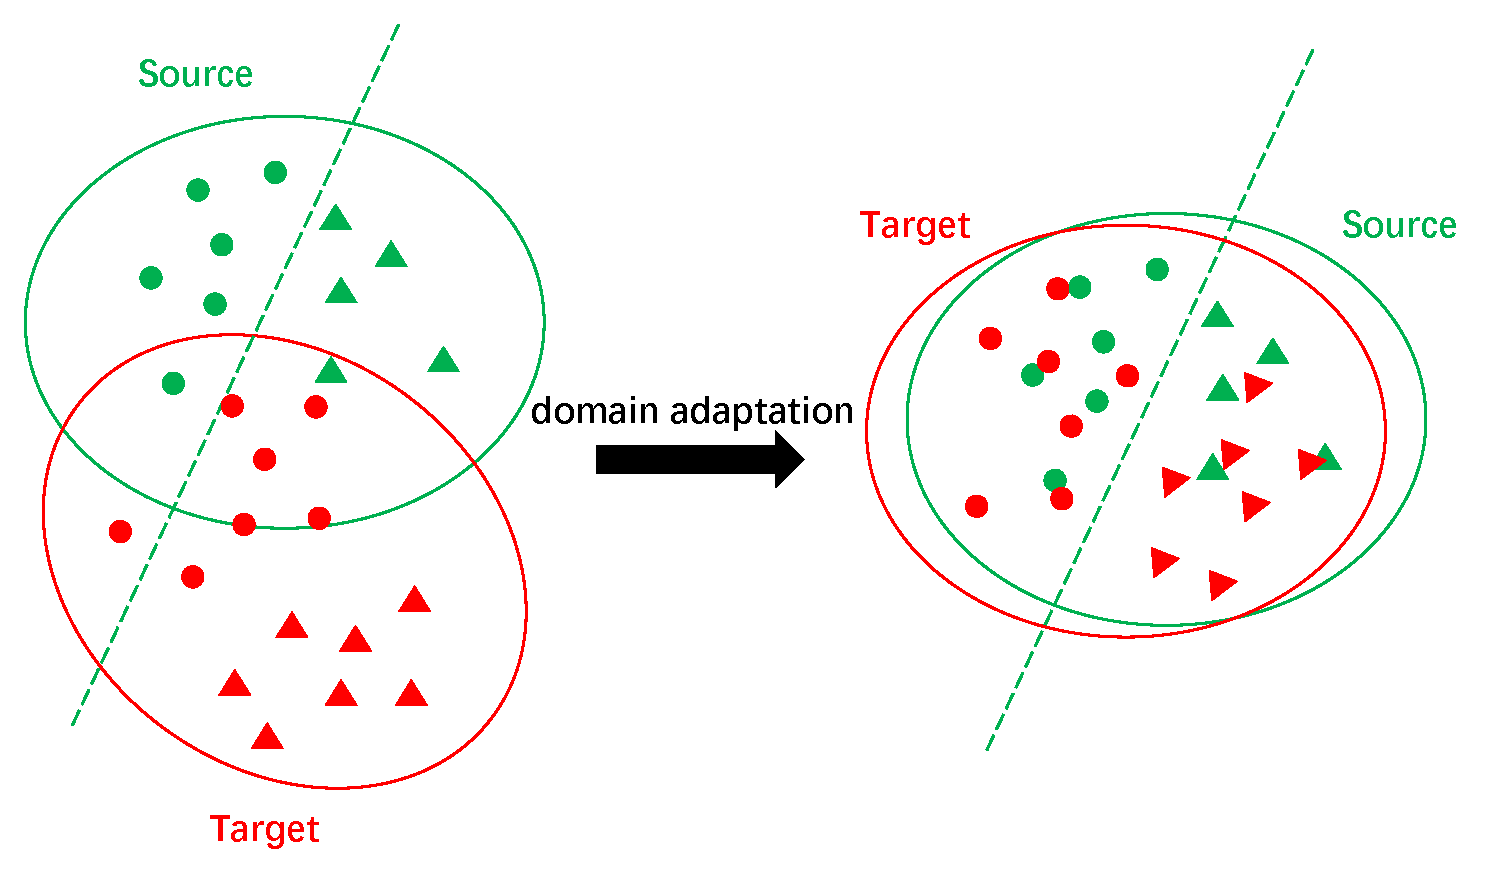
\includegraphics[width = 0.8\textwidth]{ljx/figure/2-3DA.pdf}
    \bicaption[\xiaosi 域适应]{\wuhao 域适应}{\wuhao Domain adaptation}
    \label{fig:2-3}
    % \vspace{-0.4cm} 
\end{figure}
% \vspace{-0.35cm} 
% \subsection{域对齐的典型方法}
% \subsection{基于差异度量的域对齐}

1)基于差异度量的域对齐。
% 此类方法显式定义域间分布差异,并通过优化目标函数缩小差异。常用度量包括最大均值差异(Maximum Mean Discrepancy, MMD)和对比域差异(Contrastive Domain Discrepancy, CDD)。对于常用的MMD,其计算两域在再生核希尔伯特空间(RKHS)中的均值差异,表达式如公式\eqref{eq:2-9}所示:
最大均值差异(Maximum Mean Discrepancy, MMD)是一种衡量两个分布之间差异的常用方法,尤其在域适应与生成对抗网络等任务中应用广泛。它的核心思想是先将数据映射到一个称为可再生核希尔伯特空间(Reproducing Kernel Hilbert Space, RKHS)的高维特征空间中,再比较两个分布在该特征空间中平均嵌入之间的距离。如果两个分布越相似,它们在该空间中的平均嵌入就越接近;反之则越远。$MMD$表达式如公式\eqref{eq:2-9}所示:
\begin{equation}
    \label{eq:2-9}
    MMD^2 = \left\| \frac{1}{N_s} \sum_{i=1}^{N_s} \phi(x_i^s) - \frac{1}{N_t} \sum_{j=1}^{N_t} \phi(x_j^t) \right\|_{\mathbf{H}}^2
\end{equation}
式中,$\phi(\cdot)$是将数据映射到高维空间的核函数;$N_s$,$N_t$分别是源域和目标域的样本数。通过最小化$MMD$的方式,约束模型特征提取器,使其能够学习到域不变特征知识。

2)对抗式域适应。
受生成对抗网络(Generative Adversarial Network, GAN)启发,对抗训练通过域判别器$D$引导特征生成器$g_\theta$混淆域特征,其目标函数为极小极大博弈,如公式\eqref{eq:2-10}所示:
\begin{equation}
    \label{eq:2-10}
    \min_{g_\theta} \max_{D} \mathbb{E}_{x^s}[\log D(g_\theta(x^s))] + \mathbb{E}_{x^t}[\log (1 - D(g_\theta(x^t)))]
\end{equation}
其中$D$试图区分源域与目标域特征,而$g_\theta$试图生成$D$无法区分的特征。在经典模型对抗域适应网络DANN\upcite{DANN}中,则是将对抗损失与任务损失结合,如公式\eqref{eq:2-11}所示:
\begin{equation}
    \label{eq:2-11}
    % \mathbf{L}_{\text{DANN}} = \mathbf{L}_{\text{task}} - \lambda \cdot \mathbf{L}_{\text{adv}}
    L_{DANN} = L_{task} - \lambda \cdot L_{adv}
\end{equation}

% \subsection{自训练与伪标签}
3)自训练与伪标签。
自训练利用模型对目标域的预测生成伪标签,逐步迭代优化。定义伪标签为$\hat{y}_j^t = \arg\max_c f_\theta(x_j^t)$,目标域损失表达是如公式\eqref{eq:2-12}所示:
\begin{equation}
    \label{eq:2-12}
    % \mathbf{L}_{\text{self}} = \sum_{j=1}^{N_t} \mathbb{I}(\max f_\theta(x_j^t) > \tau) \cdot \mathbf{L}(f_\theta(x_j^t), \hat{y}_j^t)
    L_{self} = \sum_{j=1}^{N_t} \mathbb{I}(\max f_\theta(x_j^t) > \tau) \cdot L(f_\theta(x_j^t), \hat{y}_j^t)
\end{equation}
式中,$\tau$为置信度阈值;$\mathbb{I}(\cdot)$为指示函数。此方法需谨慎设计阈值以避免噪声累积,常与对抗训练结合使用。

\section{数据集介绍}
% 虽然目前开源点云语义分割数据集很多,但是不同的数据集适用于不同的场景,在点云语义分割域适应任务中,通常会选择一些比较流行且大家公认的特定数据集用于进行域适应任务。本研究涉及到合成到真实以及真实到真实两个跨域场景,因此将对这两个场景下的所有数据集都进行介绍,其中合成到真实数据集一般使用合成数据SynLiDAR适应到SemanticPOSS或者emanticKITTI真实数据集上,而在真实到真实跨域场景一般使用真实数据SemanticKITTI与nuScenes进行相互迁移适应。接下来,本小节将分别对以上数据集进行介绍。
% (室外跨域任务,合成到真实常用数据集,真实到真实常用数据集,,以下小节分别对以上数据集进行介绍)
% 虽然目前已有许多开源的点云语义分割数据集,但它们往往适用于不同的应用场景。在点云语义分割的域适应任务中,通常会选择一些流行且广受认可的特定数据集作为实验标准。本研究同时涉及合成到真实(Synthetic-to-Real)和真实到真实(Real-to-Real)两个跨域场景。其中,在合成到真实的跨域场景下,通常使用合成数据SynLiDAR\upcite{xiao2022transfer}迁移至SemanticPOSS\upcite{pan2020semanticposs}或 SemanticKITTI\upcite{behley2019semantickitti}等真实数据集;而在真实到真实的跨域场景中,则一般使用SemanticKITTI与nuScenes\upcite{caesar2020nuscenes}两个真实数据集进行相互迁移适应。以上所涉及的数据集均为室外数据集,接下来本小节将分别对这些数据集进行详细介绍。
虽然目前已有许多开源的点云语义分割数据集,但它们往往针对不同的应用场景设计,具有各自的特点和局限性。在点云语义分割的域适应任务中,通常会选择一些流行且广受认可的特定数据集作为实验标准,以确保结果具有可比性和公平性。本研究同时涉及合成到真实(Synthetic-to-Real)和真实到真实(Real-to-Real)两个跨域场景。在合成到真实的跨域场景下,通常使用合成数据SynLiDAR\upcite{xiao2022transfer}作为源域数据,将其迁移至SemanticPOSS\upcite{pan2020semanticposs}或SemanticKITTI\upcite{behley2019semantickitti}等真实数据集;而在真实到真实的跨域场景中,则一般选择SemanticKITTI与nuScenes\upcite{caesar2020nuscenes}这两个主流的真实数据集进行互相迁移适应。这些数据集均主要反映室外场景的特点,如数据密度、采集角度及环境复杂性等,具有较高的代表性和挑战性。接下来,本小节将对上述数据集的采集背景、数据规模以及在跨域任务中的应用情况进行详细介绍,以便为后续实验提供坚实的数据基础。
\subsection{SynLiDAR数据集}
SynLiDAR是一个大规模的合成LiDAR点云数据集,专为促进从合成数据到真实数据的跨域语义分割研究而创建。该数据集包含超过190亿个逐点标注的点,涵盖32个语义类别,具有丰富的语义信息和高度的几何准确性。与现有的真实LiDAR数据集相比,SynLiDAR的规模更大,质量更高,语义类别更丰富,且标注更加细致和全面。SynLiDAR的点云数据是在多个由专业3D设计师构建的虚拟环境中生成的,这些虚拟环境包含大量与真实世界数据在几何形状和布局上相似的物体模型。如图\ref{fig:2-4}所示,数据集中的每个虚拟场景都经过精心设计,以确保合成数据的高质量和真实性。SynLiDAR的点云数据具有逐点标注,标注类别包括汽车、自行车、摩托车、卡车、其他车辆、行人、骑自行车者、骑摩托车者、道路、停车场、人行道、其他地面、建筑物、围栏、植被、树干、地形、杆、交通标志等,涵盖了丰富的动静态对象,适用于多种语义分割任务。
\vspace{-0.1cm}
\begin{figure}[h]
    \centering
    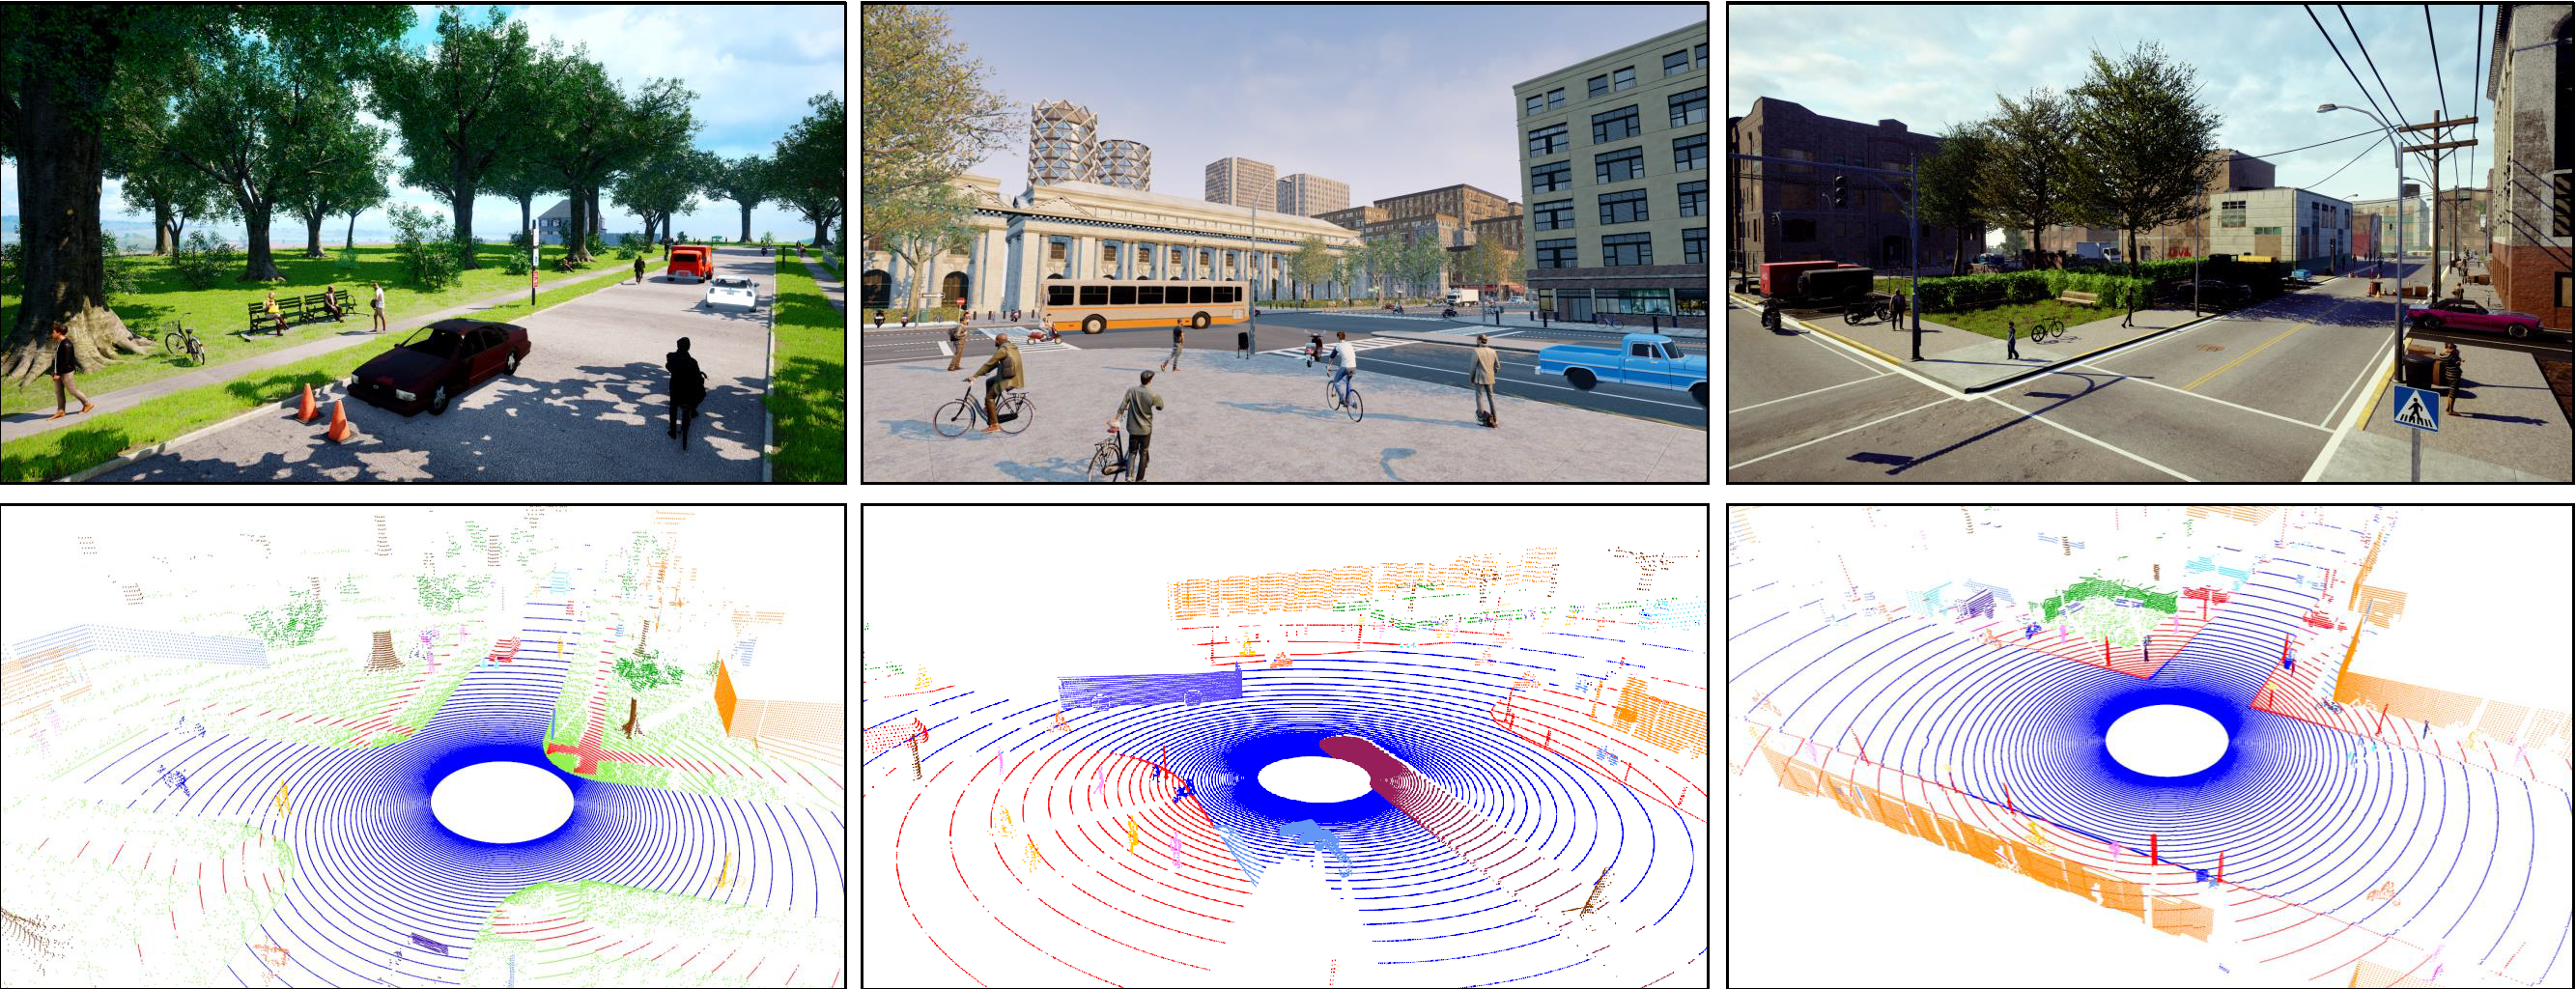
\includegraphics[width = 1\textwidth]{ljx/figure/2-5/synlidar.png}
    \bicaption[\xiaosi SynLiDAR数据集\upcite{xiao2022transfer}]{\wuhao SynLiDAR数据集\upcite{xiao2022transfer}}{\wuhao SynLiDAR datasets\upcite{xiao2022transfer}}
    \label{fig:2-4}
\end{figure}
\vspace{-0.35cm} 
\subsection{SemanticKITTI数据集}
SemanticKITTI是一个大规模的室外数据集,是基于真实道路场景构建的激光雷达点云数据集,可用于多种点云分割任务和语义场景补全,与SemanticPOSS相比,该数据集场景更广泛且庞大。其数据通过车载激光雷达采集,包含三维坐标与反射强度信息,但未包含颜色特征。数据集基于 KITTI里程计基准扩展,通过逐点标注实现了360度全景点云的精细化语义标注,涵盖动态与静态对象19个类目标,同时包含地面与可行驶区域等特殊语义类别。
% 涵盖19类目标,包括行人、骑行者、轿车、卡车、道路、人行道、停车场、建筑物、植被、树干、栅栏、杆状物、交通标志等动态与静态对象,同时包含地面与可行驶区域等特殊语义类别。
如图\ref{fig:2-6}所示,数据集共由22个点云序列组成,每个序列都包含一段录制点云。其中,序列00$\sim$10和08总共提供了23201个有标注信息的点云,分别用于训练和验证;11$\sim$21 提供了20351个没有标注信息的点云,用于测试。
点云语义分割域适应中,将SynLiDAR数据集上训练的模型迁移到SemanticKITTIT数据集上,并将类别映射为19个共有的语义类别,包括汽车、自行车、摩托车、卡车、其他车辆、行人、骑自行车者、骑摩托车者、道路、停车场、人行道、其他地面、建筑物、栅栏、植被、树干、地形、杆状物、交通标志。
\vspace{-0.1cm}
\begin{figure}[H]
    \centering
    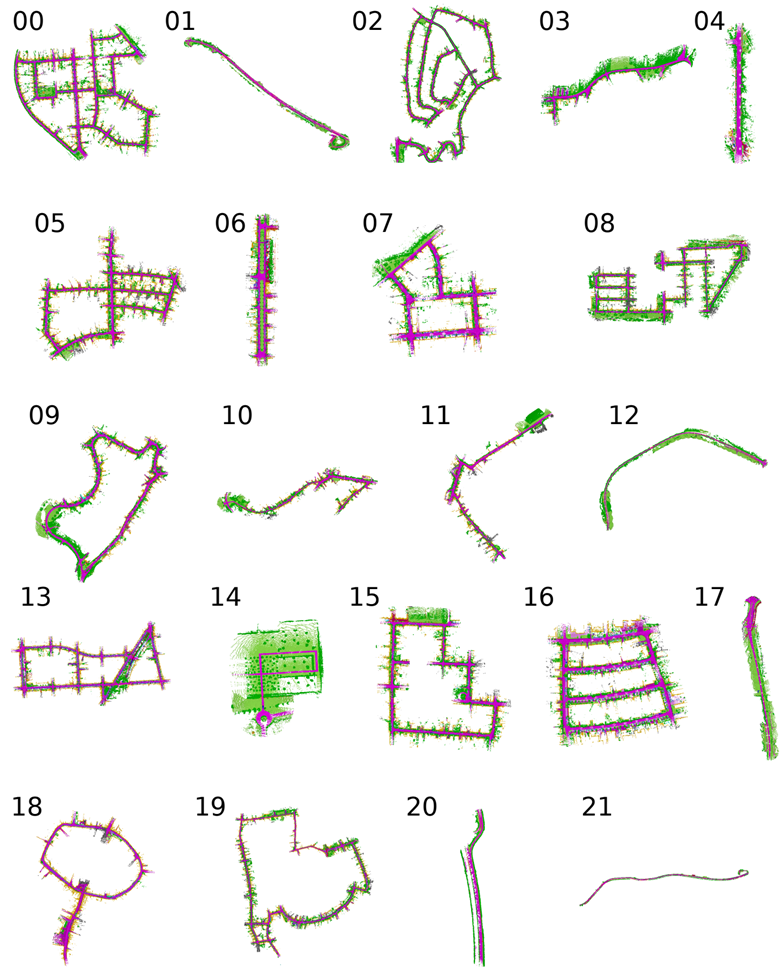
\includegraphics[width = \textwidth, scale=0.5]{ljx/figure/2-5/kitti.png}
    \bicaption[\xiaosi SemanticKITTI数据集\upcite{behley2019semantickitti}]{\wuhao SemanticKITTI数据集\upcite{behley2019semantickitti}}{\wuhao SemanticKITTI datasets\upcite{behley2019semantickitti}}
    \label{fig:2-6}
\end{figure}
\vspace{-0.35cm} 
\subsection{SemanticPOSS数据集}
SemanticPOSS是一个真实世界的小规模数据集,使用Pandora 40线激光雷达传感器在北京大学采集,包含2988个扫描样本。每个扫描样本包含约80,000到100,000个点,捕捉了典型的都市户外场景。该数据集包含13个语义类别,为研究者提供了丰富的数据资源。在数据集划分方面,遵循先验研究的方法,将包含500个点云样本的03序列分配用于验证,而剩余的2488个点云样本则用于训练。在点云语义分割域适应中,将SynLiDAR数据集上训练的模型迁移到SemanticPOSS数据集上,并将类别映射为13个共有的语义类别,包括汽车、自行车、人、骑行者、地面、建筑物、栅栏、植物、树干、杆、交通标志、垃圾桶、路锥/石块。其数据集展示图如图\ref{fig:2-5}所示。
% \vspace{-0.1cm}
\begin{figure}[h]
    \centering
    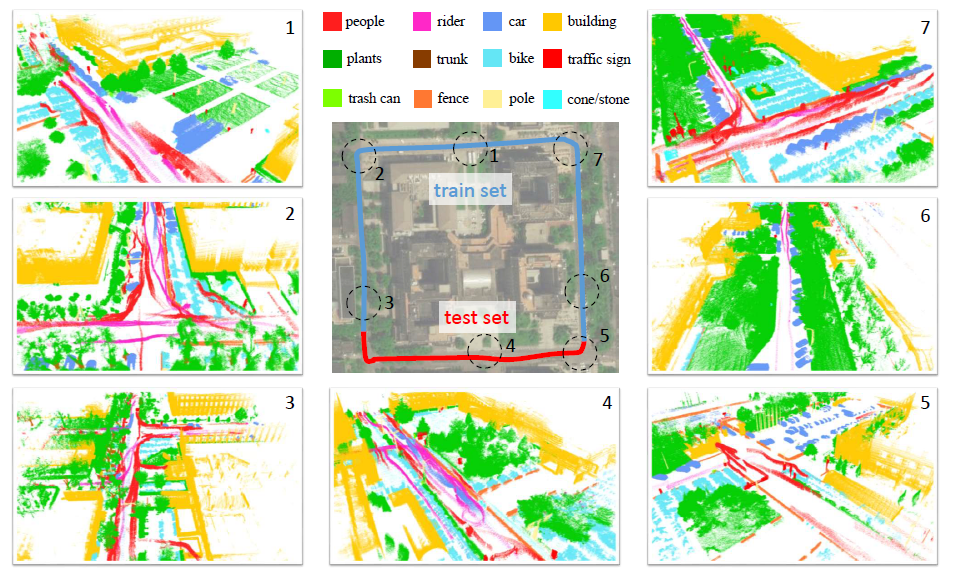
\includegraphics[width = \textwidth, scale=0.5]{ljx/figure/2-5/poss.png}
    \bicaption[\xiaosi SemanticPOSS数据集\upcite{pan2020semanticposs}]{\wuhao SemanticPOSS数据集\upcite{pan2020semanticposs}}{\wuhao SemanticPOSS datasets\upcite{pan2020semanticposs}}
    \label{fig:2-5}
    \vspace{-0.5cm} 
\end{figure}
\subsection{nuScenes数据集}
nuScenes是多模态自动驾驶数据集的代表性资源,整合了激光雷达、摄像头、毫米波雷达及定位系统的同步采集数据,覆盖波士顿与新加坡的1,000个复杂驾驶场景。其激光雷达语义分割子集(nuscenes-lidarseg)包含约14亿个点云,总计40,000帧数据,划分为850个训练验证场景与150个测试场景。语义标注涵盖16类关键目标,包括自行车、公交车、轿车、工程车、摩托车、行人、卡车、拖车等交通参与者,可行驶区域、其他人造地面、人行道、自然地面等道路要素,以及障碍物、锥形路标、植被和人造物体等环境元素。类别设计注重实际驾驶场景的多样性,尤其强调对临时障碍物的精细化标注,例如锥形路标与非铺装路面,为复杂环境下的多目标感知与路径规划提供高精度数据支持。其数据集展示图如图\ref{fig:2-7}所示。
在点云语义分割域适应中,SemanticKITTIT与nuScenes数据进行模型的相互迁移,最终将类别映射为7个共有的语义类别,包括车辆、行人、道路、人行道、地形、人造物体、植被。
\vspace{-0.1cm}
\begin{figure}[h]
    \centering
    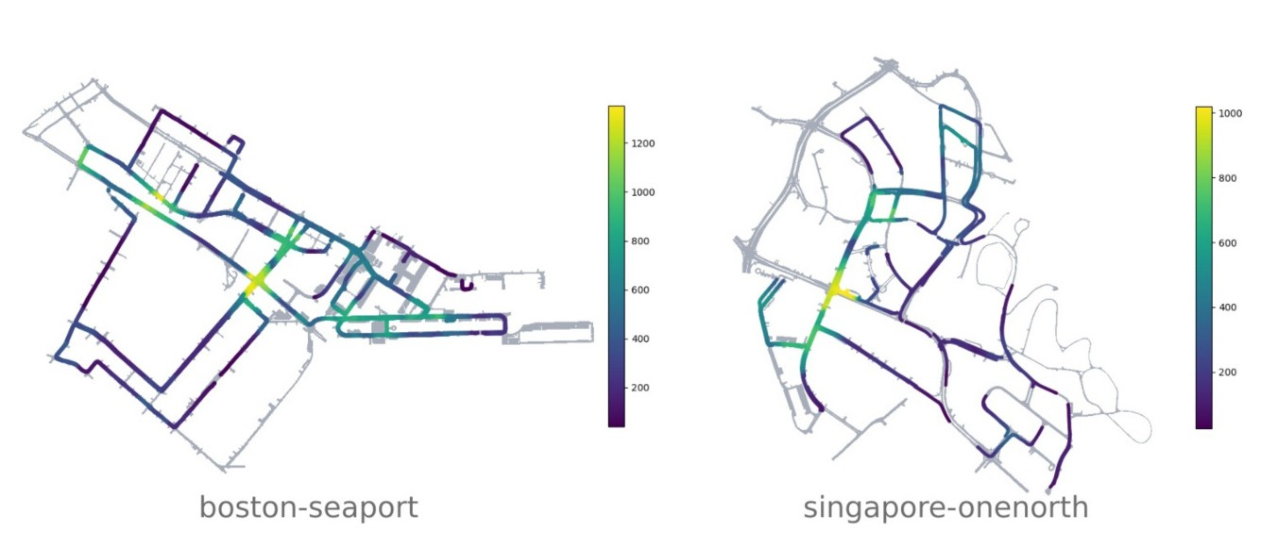
\includegraphics[width = \textwidth, scale=0.5]{ljx/figure/2-5/nuScenes.pdf}
    \bicaption[\xiaosi nuScenes数据集\upcite{caesar2020nuscenes}]{\wuhao nuScenes数据集\upcite{caesar2020nuscenes}}{\wuhao nuScenes datasets\upcite{caesar2020nuscenes}}
    \label{fig:2-7}
\end{figure}
\vspace{-0.35cm} 
\section{本章小结}
本章主要对点云语义分割主动域适应相关领域的基础知识做了全面介绍,包含对点云语义分割,主动学习,域适应在内的多个不同领域分别做了介绍。 对于点云语义分割的相关基础知识,首先详细介绍了点云的获取方式、点云的特征以及室内外点云的差异。根据特征提取方式的不同,进一步对点云语义分割任务的基本模型和基本实现方式做了基础介绍,最后还介绍了语义分割任务中常用的评价指标mIoU。对于主动学习相关基础知识,主要对主动学习方法的基本概念和基本流程做了详细阐述;针对域适应基础知识,首先介绍了域适应的概念、目的以及任务,接着又对常见的域对齐方法进行了梳理和解释。最后还对点云语义分割域适应任务中常用的室外跨域数据集分别进行了介绍。本章介绍的各方面基础知识对后续章节中算法设计的阅读理解起到重要铺垫作用。
% 可在此增加文字以增加页数